\documentclass{article}

\usepackage{url} 

\usepackage{pdfpages}
\usepackage{lastpage}
\usepackage{fancyhdr}
\usepackage{ngerman}
\usepackage{listings}

\usepackage{tabularx}
\usepackage{floatrow}
\usepackage[tableposition=top]{caption}
\floatsetup[table]{capposition=top}

\usepackage{amsmath, amssymb}

\usepackage[utf8]{inputenc}

\usepackage{xifthen}
\usepackage[numbib]{tocbibind}



\newcommand\twodigits[1]{%
   \ifnum#1<10 0#1\else #1\fi
}



\lhead{Signalleitung}
\rhead{20. November 2020\\T. Maier, J. Winkler}
%\cfoot{\twodigits{\thepage}~/ \pageref{LastPage}}
\cfoot{{\thepage}~/ \pageref{LastPage}}

\newcommand{\W}{\text{W}}
\newcommand{\V}{\text{V}}
\newcommand{\A}{\text{A}}


\newcommand{\mini}{\operatorname{min}}


\begin{document}

\parindent0cm


\includepdf{Deckblatt.pdf}


\pagestyle{fancy}

\tableofcontents
\newpage
\section{Aufgabenstellung}

\begin{enumerate}
\item Messung und Erklärung des zeitlichen Spannungsverlaufes am Anfang und Ende eines etwa 25-30 m langen Koaxialkabels für angelegte Spannungspulse in folgenden Fällen:
\begin{enumerate}
\item angepasster Innenwiderstand der Signalquelle.
\item Signalquelle mit hohem Innenwiderstand.
\item Signalquelle mit niedrigem Innenwiderstand.
\end{enumerate}
\item Bestimmung des Reflexionskoeffizienten des Kabelendes als Funktion des Abschlusswiderstandes und Bestimmung der Kabelimpedanz.
\item Bestimmung der Signalgeschwindigkeit im Koaxialkabel. Aus dem Ergebnis ist die relativePermittivität des Isolatormaterials des Koaxialkabels zu ermitteln.
\item Ein Verzweiger dient dazu, das Signal einer Quelle auf mehrere Empfänger aufzuteilen, ohne dass das Signal durch die Aufteilung gestört wird. Aufgabe: Dimensionierung der Wi-derstände für einen passiven, symmetrischen Verzweiger und experimentelle Demonstrationder Funktion der Schaltung.
 
\end{enumerate}



\section{Voraussetzungen und Grundlagen}

Bei Signalen in Kabeln wird am Ende des Kabels ein Teil reflektiert und ein Teil transmittiert. Nach Kirchhoff gilt
\begin{align}
U_e + U_r &= U_t \\
I_e - I_r &= I_t
\end{align}
Variablen mit $e$ als Subskript beziehen sich immer auf ein einlaufendes Signal, während $r$ für reflektiert und $t$ für transmittiert steht.

Es wird zusätzlich noch der Reflexionskoeffizient benötigt, welcher definiert ist als
\begin{align}
\rho = \frac{U_r}{U_e}
\end{align}
Durch die Impedanz des Kabels $Z_K = \dfrac{U_e}{I_e} = \dfrac{U_r}{I_r}$ und vom Anschluss $Z_A = \dfrac{U_t}{I_t}$ folgt für den Reflexionskoeffizienten
\begin{align}
\rho = \frac{Z_A-Z_K}{Z_A+Z_K}
\end{align}





%\begin{figure}[H]
%\caption{Transformator}
%\label{fig:transformator}
%{\centering
%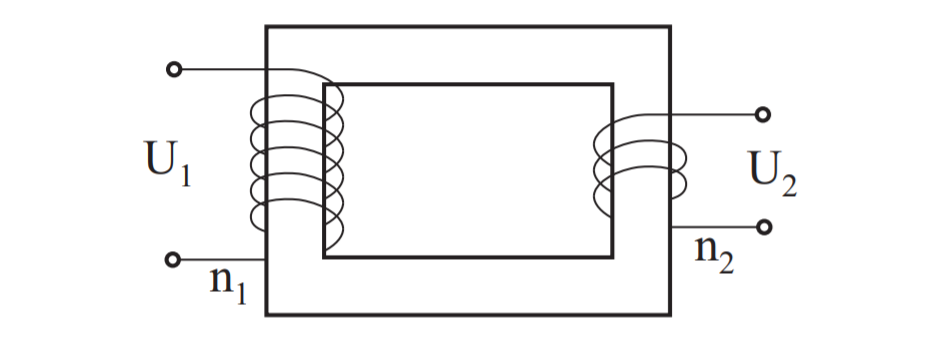
\includegraphics[scale=0.4]{transformator.png}
%~
%}
%\end{figure}

%\newcommand{\R_eins}{R1 $ =(12.00\pm0.12)~\Omega$}
\newcommand{\ifequals}[3]{\ifthenelse{\equal{#1}{#2}}{#3}{}}
\newcommand{\case}[2]{#1 #2} 
\newenvironment{switch}[1]{\renewcommand{\case}{\ifequals{#1}}}{}


\newcommand{\R}[1]{
\begin{switch}{#1}
\case{1}{R1 $ =(1794 \pm 18)~\Omega$}%
\case{2}{R2 $ =(1195 \pm 12)~\Omega$}%
\case{3}{R3 $ =(676.6\pm 6.8)~\Omega$}%
\case{4}{R4 $ =(330.36\pm3.30)~\Omega$}%
\case{5}{R5 $ =(179.80\pm0.68)~\Omega$ }%
\case{6}{R6 $ =(100.40 \pm 1.00 )~\Omega$}%
\case{7}{R7 $ =(68.40 \pm 0.68)~\Omega$}%
\case{8}{R8 $ =(47.60\pm 0.47)~\Omega$ }%
\case{9}{R9 $ =(33.30 \pm 0.33)~\Omega$}%
\case{10}{R10 $ =(12.40\pm 0.12)~\Omega$}%
\case{11}{R11 $ =(18.32\pm 0.18)~\Omega$}%
\end{switch}}

\section{Geräteliste}

\begin{table}[H]
\caption{Liste der verwendeten Geräte}

~

\begin{tabular}{l|p{3cm}p{3.5cm}llll}
Abk. & Typ    & Daten & Inv.Nr.  \\
\hline
O & Oszilloskop  DSO-X 2022A \\
FG1 & Frequenzgenerator  BK precision 4063 &   \\
K1 & Koaxialkabel 1  & $\ell_2=(0.50\pm 0.01)~$m \\
K2 & Koaxialkabel 2  & $\ell_3=(X\pm 0.01)~$m \\
 R1 & Widerstand &  \R1 \\
R2 & Widerstand & \R2 \\
R3 & Widerstand & \R3 \\
R4 & Widerstand & \R4 \\
R5 & Widerstand & \R5 \\
R6 & Widerstand & \R6 \\
R7 & Widerstand & \R7 \\
R8 & Widerstand & \R8 \\
R9 & Widerstand & \R9 \\
R10 & Widerstand & \R{10} \\
R11 & Widerstand & \R{11}
\end{tabular}
\end{table}






\section{Beschreibung der Versuchsanordnung}

Im ersten Teil der wird der zeitliche Spannungsverlauf am Anfang und Ende des Kabels gemessen. Dabei variiert der Innenwiderstand der Signalquelle. Die Abbildungen \ref{fig:anordnung_task1a}, \ref{fig:anordnung_task1b} und \ref{fig:anordnung_task1c} beschreiben den Aufbau.


\begin{figure}[H]
\centering
\caption{Versuch 1 (a): Signalquelle (FG1) ist mit dem zu testenden Koaxialkabel verbunden. CH1 des Oszilloskops misst den Spannungsverlauf am Anfang des Kabels und CH2 am Ende.}
\label{fig:anordnung_task1a}
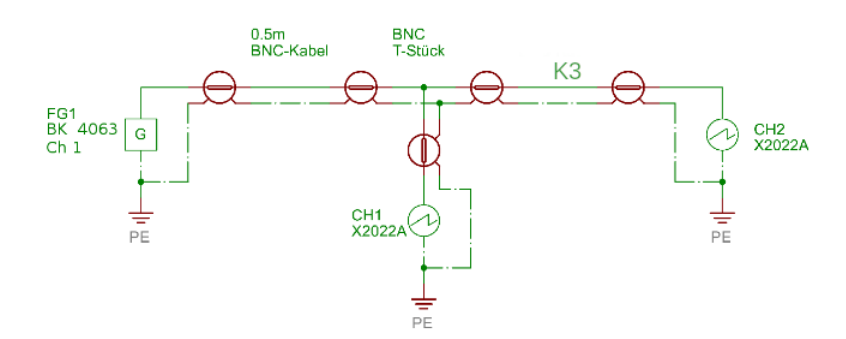
\includegraphics[scale=1.6]{task1a.png}
\end{figure}


\begin{figure}[H]
\centering
\caption{Versuch 1 (a) als Foto. Die Kurven am Oszilloskop zeigen die Daten aus Grafik~\ref{fig:task1a_100ns}.}
\label{fig:foto_task1a}
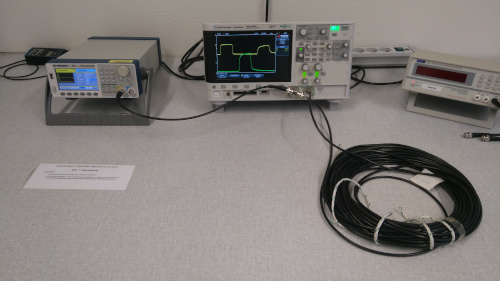
\includegraphics[scale=0.6]{foto_task1a.jpg}
\end{figure}



\begin{figure}[H]
\centering
\caption{Versuch 1 (b): Signalquelle (FG1) ist mit dem zu testenden Koaxialkabel verbunden. Erhöhung des Innenwiderstandes von FG1 durch in Serie geschalteten Widerstand. CH1 des Oszilloskops misst den Spannungsverlauf am Anfang des Kabels und CH2 am Ende.}
\label{fig:anordnung_task1b}
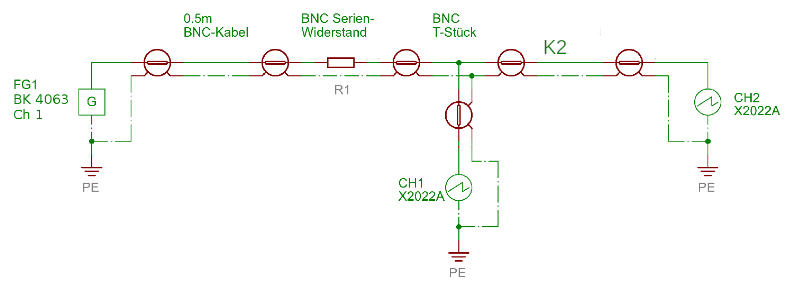
\includegraphics[scale=2]{task1b.png}
\end{figure}



\begin{figure}[H]
\centering
\caption{Versuch 1 (b) als Foto. Die Kurven am Oszilloskop zeigen die Daten aus Grafik \ref{fig:task1b_2300ns}.}
\label{fig:foto_task1b}
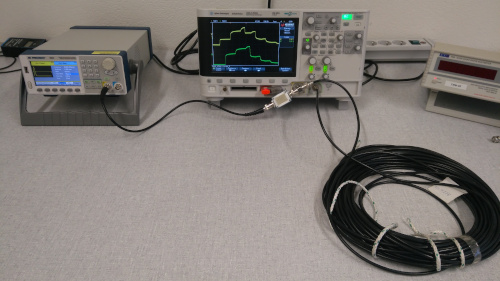
\includegraphics[scale=0.6]{foto_task1b.jpg}
\end{figure}



\begin{figure}[H]
\centering
\caption{Versuch 1 (c): Signalquelle (FG1) ist mit dem zu testenden Koaxialkabel verbunden. Senkung des Innenwiderstandes von FG1 durch parallel geschalteten Widerstand. CH1 des Oszilloskops misst den Spannungsverlauf am Anfang des Kabels und CH2 am Ende.}
\label{fig:anordnung_task1c}
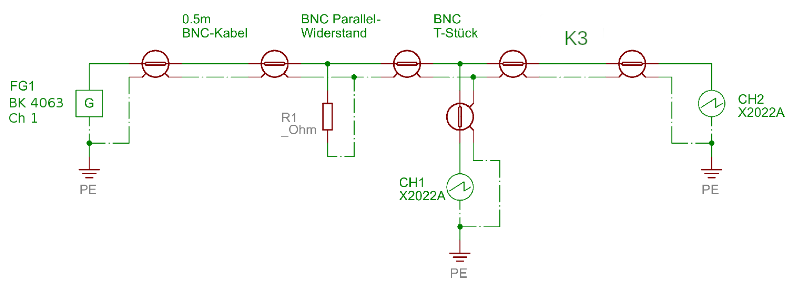
\includegraphics[scale=2]{task1c.png}
\end{figure}



\begin{figure}[H]
\centering
\caption{Versuch 1 (c) als Foto. Die Kurven am Oszilloskop zeigen die Daten aus Grafik \ref{fig:task1c_150ns}.}
\label{fig:foto_task1b}
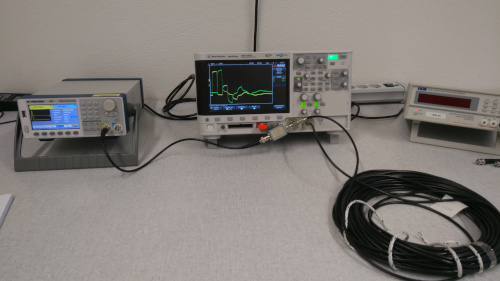
\includegraphics[scale=0.6]{foto_task1c.jpg}
\end{figure}


\begin{figure}[H]
\centering
\caption{Versuch 2: Signalquelle (FG1) ist mit dem zu testenden Koaxialkabel verbunden. CH1 des Oszilloskops misst den Spannungsverlauf am Anfang des Kabels. Am Ende des Kabels befindet sich ein Widerstand. Durch diesen Aufbau kann der Reflexionskoeffizient gemessen werden.}
\label{fig:anordnung_task2}
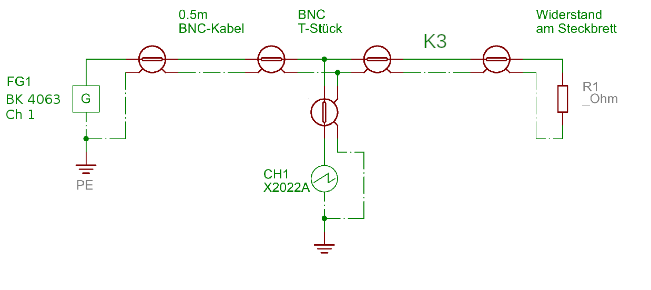
\includegraphics[scale=2]{task2.png}
\end{figure}


\begin{figure}[H]
\centering
\caption{Versuch 4: Aufbau eines symmetrischen Verzweigers. $R$ ist so zu wählen, dass keine Reflexionen auftreten.}
\label{fig:anordnung_task4}
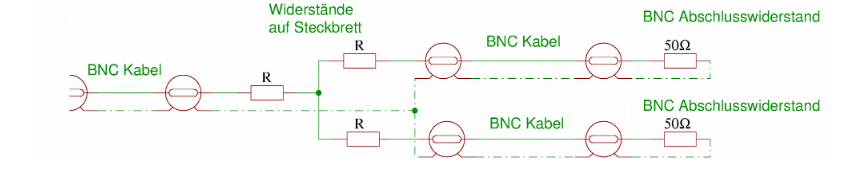
\includegraphics[scale=2]{task4.png}
\end{figure}


\section{Versuchsdurchführung und Messwerte}

\subsection{Zeitlicher Spannungsverlauf an den Enden des Koaxialkabels}

\subsubsection{Angepasster Innenwiderstand}

Der Versuchsaufbau ist in Abbildung~\ref{fig:anordnung_task1a} beschrieben bzw. in Abbildung~\ref{fig:foto_task1a} als Foto dargestellt. Der Frequenzgenerator wird auf \texttt{Pulse} mit einer Frequenz von 30~kHz eingestellt. Zusätzlich wird \texttt{PulseWidth} auf $100~$ns, $240~$ns, $500~$ns und $750~$ns gesetzt.



\begin{figure}[H]
\centering
\caption{Spannungsverlauf an beiden Enden des Koaxialkabels mit $t_p=100$~ns.}
\label{fig:task1a_100ns}
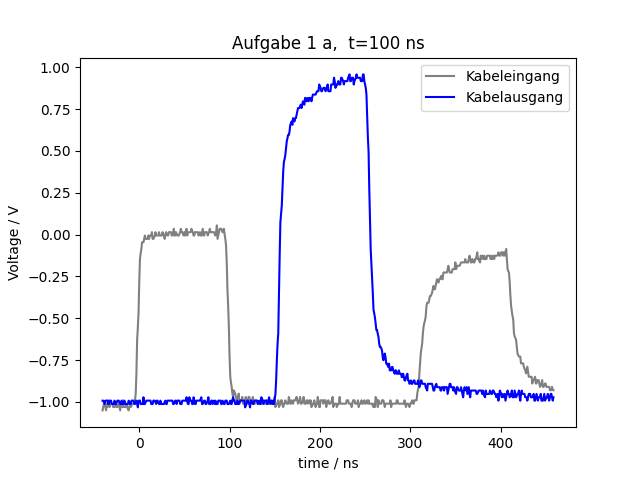
\includegraphics[scale=0.6]{bilder/task1a/task1a_100ns.png}
\end{figure}

\begin{figure}[H]
\centering
\caption{Spannungsverlauf an beiden Enden des Koaxialkabels mit $t_p=240$~ns.}
\label{fig:task1a_240ns}
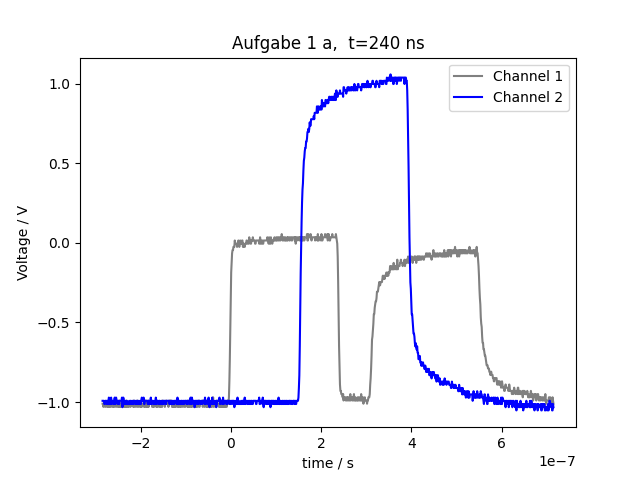
\includegraphics[scale=0.6]{bilder/task1a/task1a_240ns.png}
\end{figure}

\begin{figure}[H]
\centering
\caption{Spannungsverlauf an beiden Enden des Koaxialkabels mit $t_p=500$~ns.}
\label{fig:task1a_500ns}
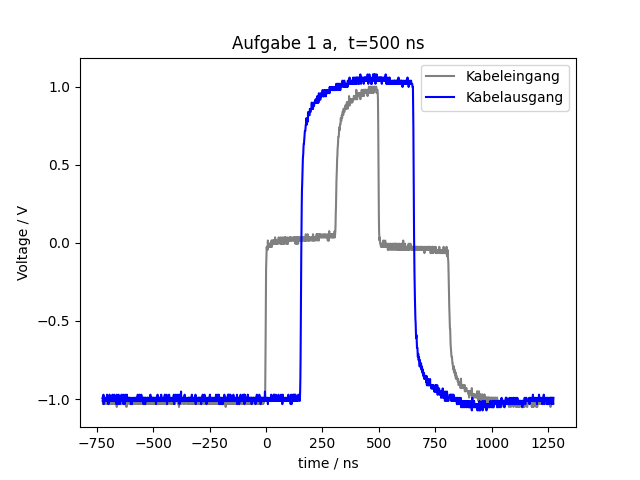
\includegraphics[scale=0.6]{bilder/task1a/task1a_500ns.png}
\end{figure}

\begin{figure}[H]
\centering
\caption{Spannungsverlauf an beiden Enden des Koaxialkabels mit $t_p=750$~ns.}
\label{fig:task1a_750ns}
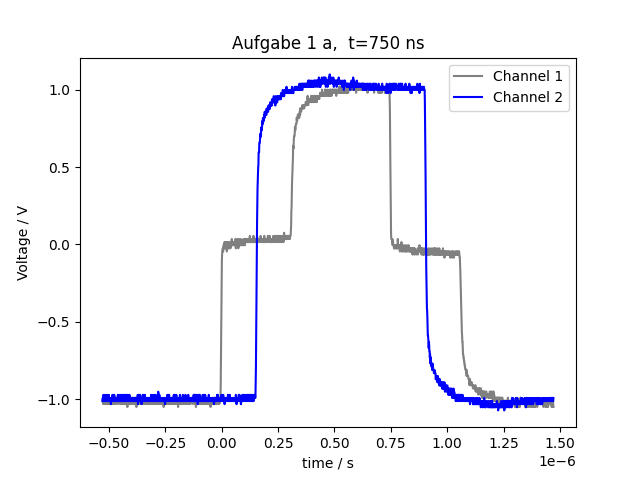
\includegraphics[scale=0.6]{bilder/task1a/task1a_750ns.png}
\end{figure}





\subsubsection{Hoher Innenwiderstand}
Der Versuchsaufbau ist in Abbildung~\ref{fig:anordnung_task1b} beschrieben. Hier soll ein Puls $t_p = 150~$ns und einmal $t_p = 2.3~\mu$s  als Signal verwendet werden.


\begin{figure}[H]
\centering
\caption{Spannungsverlauf an beiden Enden des Koaxialkabels. Hoher Innenwiderstand der Singalquelle. Channel 1 ist Spannung am Beginn des Kabels, Channel 2 am Ende. $t_p = 150~$ns.}
\label{fig:task1b_150ns}
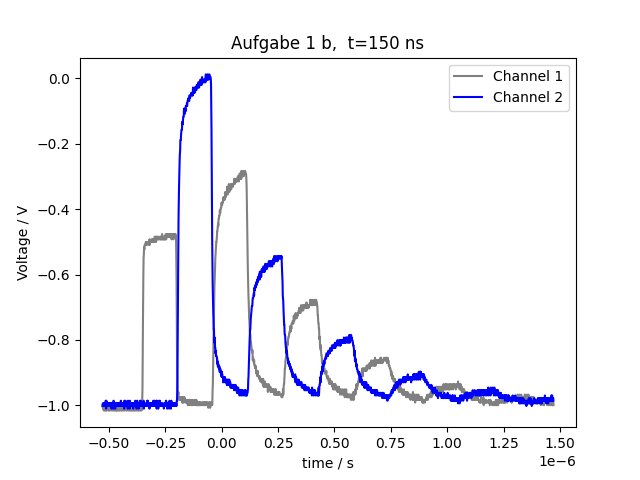
\includegraphics[scale=0.6]{bilder/task1b/task1b_150ns.png}
\end{figure}

\begin{figure}[H]
\centering
\caption{Spannungsverlauf an beiden Enden des Koaxialkabels. Hoher Innenwiderstand der Singalquelle. Channel 1 ist Spannung am Beginn des Kabels, Channel 2 am Ende. $t_p = 2.3~\mu$s.}
\label{fig:task1b_2300ns}
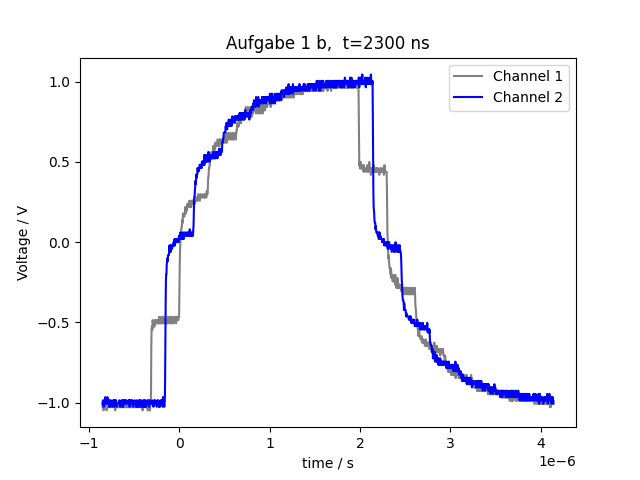
\includegraphics[scale=0.6]{bilder/task1b/task1b_2300ns.png}
\end{figure}



\subsubsection{Niedriger Innenwiderstand}
Der Versuchsaufbau ist in Abbildung~\ref{fig:anordnung_task1c} beschrieben. Hier soll ein Puls $t_p = 150~$ns und einmal $t_p = 2.65~\mu$s  als Signal verwendet werden.

\begin{figure}[H]
\centering
\caption{Spannungsverlauf an beiden Enden des Koaxialkabels. Niedriger Innenwiderstand der Singalquelle. Channel 1 ist Spannung am Beginn des Kabels, Channel 2 am Ende. $t_p = 150$ns.}
\label{fig:task1c_150ns}
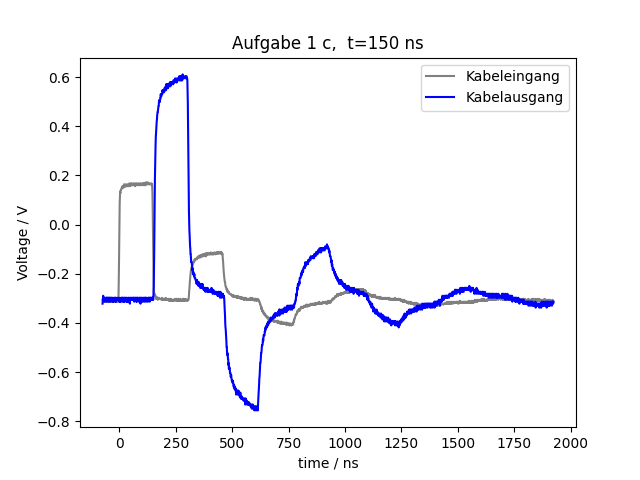
\includegraphics[scale=0.6]{bilder/task1c/task1c_150ns.png}
\end{figure}

\begin{figure}[H]
\centering
\caption{Spannungsverlauf an beiden Enden des Koaxialkabels. Niedriger Innenwiderstand der Singalquelle. Channel 1 ist Spannung am Beginn des Kabels, Channel 2 am Ende. $t_p = 2.65~\mu$s.}
\label{fig:task1b_2650ns}
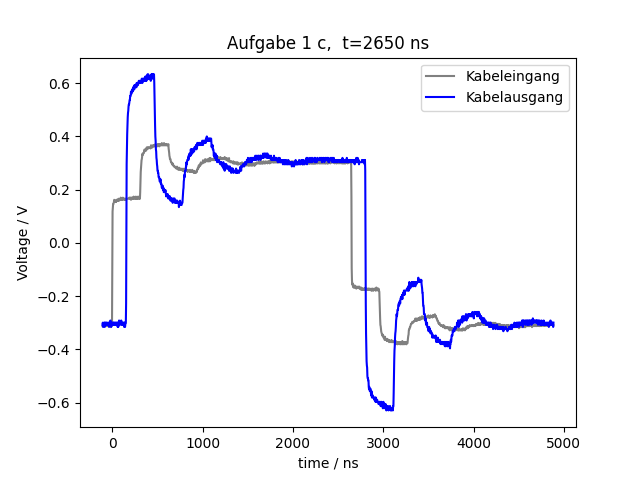
\includegraphics[scale=0.6]{bilder/task1c/task1c_2650ns.png}
\end{figure}



\subsection{Bestimmung des Reflexionskoeffizienten}

Der Versuchsaufbau ist in Grafik~\ref{fig:anordnung_task2} beschrieben.

Analog zur vorherigen Aufgabe, wurde die Frequenz wurde auf 30~kHz gestellt und die Pulszeit $t_p = 1~\mu$s. Jetzt stehen 11 verschiedene Widerstände zur Verfügung (siehe Geräteliste), welche jeweils als Abschlusswiderstand des Kabels genutzt werden.

Im Gegensatz zu Aufgabe 1 wird hier nur die Eingangsspannung gemessen. Der Eingangswiderstand der Signalquelle ist angepasst, so wie in 1 (a). Am Ende des Kabels werden verschiedene Widerstände angeschlossen. Der Spannungsverlauf dieser Widerstände wird in den Grafiken~\ref{fig:task2_R1} bis \ref{fig:task2_R11} dargestellt.





\subsection{Bestimmung der Signalgeschwindigkeit}

Hierbei wird ein Puls augesendet und jene Zeit gemessen, bis der reflektierte Impuls ankommt.


\subsection{Symmetrischer Verzweiger}


\section{Auswertung}

\subsection{Zeitlicher Spannungsverlauf an den Enden des Koaxialkabels}

\subsubsection{Angepasster Innenwiderstand}
Die Grafiken \ref{fig:task1a_50ns} bis \ref{fig:task1a_1000ns} beschreiben das Ergebnis. Nachdem das Signal durch das Kabel läuft, wird es am Ende reflektiert. Das Signal überlagert sich mit dem reflektiertem Signal und es entsteht Interferenz. Durch den angepassten Innenwiderstand in der Signalquelle wird das Signal nicht mehrfach reflektiert. 



\subsubsection{Hoher Innenwiderstand}

Durch den hohen Innenwiderstand ist am Anfang des Kabels eine stärkere Reflexion zu beobachten. Durch die stärkere Reflexion sieht man, dass eine \textit{Treppenfunktion} entsteht, da sich die Signale mehrfach im Kabel hin und her bewegen und sich ständig überlagern. Da die höhe der Treppen immer kleiner wird, lässt sich darauf schließen, dass das Signal beim mit mehrmaligem Vor- und Zurücklauf kontinuierlich abgeschwächt wird.

\subsubsection{Niedriger Innenwiderstand}



\subsection{Bestimmung des Reflexionskoeffizienten}

\subsection{Bestimmung der Signalgeschwindigkeit}

Der elektrische Impuls legt den Weg $s = 2\cdot \ell_3$ zurück. Wenn dafür die Zeit $t$ benötigt wird, dann gilt insgesamt mit Größtfehlermethode
\begin{align*}
c = \left(\frac{2\cdot \ell_3}{t} \pm \left|\frac{2\cdot \Delta \ell_3}{t} + \frac{2\cdot \ell_3}{t^2}\cdot \Delta t\right|\right)
\end{align*}

Die relative Permittivität des des Isoliermaterials ist hier außerdem zu breechnen. Aus $\varepsilon \cdot \mu = \frac{1}{c^2}$ folgt inklusive Fehleranalyse
\begin{align*}
\varepsilon_r = \frac{1}{c^2\cdot \mu\cdot \varepsilon_0} \pm \left| \frac{\Delta c}{c^3\cdot \mu\cdot \varepsilon_0} \right|
\end{align*}
mit der elektrischen Feldkonstanten $\varepsilon_0$, $\mu = \mu_r\cdot\mu_0$ und $\mu_r=1$.

\subsection{Symmetrischer Verzweiger}




\section{Diskussion}






\section{Zusammenfassung}




%\newpage 
%\appendix
%\section{Python Skript}



\definecolor{commentgreen}{RGB}{2,112,10}
\definecolor{eminence}{RGB}{108,48,130}
\definecolor{weborange}{RGB}{255,165,0}
\definecolor{frenchplum}{RGB}{129,20,83}

\lstdefinelanguage{python}{
    morekeywords={def, for, range, abs, return},
    otherkeywords={<-,->, |>, \%\{, \}, \{, \, (, )},
    sensitive=true,
    morecomment=[l]{\#},
    morecomment=[n]{/*}{*/},
    morecomment=[s][\color{purple}]{:}{\ },
    morestring=[s][\color{orange}]"",
    commentstyle=\color{commentgreen},
    keywordstyle=\color{eminence},
    stringstyle=\color{red},
	basicstyle=\ttfamily,
	breaklines,
	showstringspaces=false,
	frame=tb
}
%\lstinputlisting[language=Python,captionpos=b, label=lst:test,caption={Python Skript}]{generate_numbers.py}

%\lstinputlisting[language=Python,captionpos=b, label=lst:test,caption={Bessel Auswertung}]{generate_numbers_bessel.py}


%\lstinputlisting[language=Python,captionpos=b, label=lst:test,caption={Zerstreuungslinse Auswertung}]{generate_numbers_zerstreuungslinse.py}


\begin{thebibliography}{9}
\bibitem{moodle} Unterlagen aus Moodle, A. Hohenau, bereitgestellt von der KF Universität Graz.
\end{thebibliography}


\end{document}
